\documentclass{article}
\usepackage[utf8]{inputenc}
\usepackage{graphicx}
\usepackage{amsmath}
\usepackage{hyperref}
\usepackage{booktabs}
\usepackage{float}

\title{Análisis Estadístico de un Dataset}
\author{Tu Nombre}
\date{\today}

\begin{document}

\maketitle

\tableofcontents
\newpage

% --- Sección 1: Introducción ---
\section{Introducción}
\subsection{Contexto del Problema}
Breve descripción del contexto y los objetivos del análisis. ¿Por qué es importante este dataset? ¿Qué preguntas se buscan responder?

\subsection{Descripción del Dataset}
Información general sobre el dataset:
\begin{itemize}
    \item Fuente de los datos.
    \item Número de filas y columnas.
    \item Variables principales y su tipo (numérica, categórica, etc.).
\end{itemize}

% --- Sección 2: Análisis Exploratorio de Datos (EDA) ---
\section{Análisis Exploratorio de Datos (EDA)}
\subsection{Limpieza de Datos}
\begin{itemize}
    \item Manejo de valores faltantes.
    \item Tratamiento de outliers.
    \item Corrección de inconsistencias.
\end{itemize}

\subsection{Análisis Descriptivo}
    \subsubsection{Estadísticas descriptivas (media, mediana, desviación estándar, etc.).}


\begin{table}[H]
    \centering
    \begin{tabular}{|l|r|}
    \hline
    \textbf{Estadística} & \textbf{Valor} \\
    \hline
    Duración Media & 99.528 \\
    Duración Mediana & 98.000 \\
    Moda de la Duración & 90.000 \\
    Varianza (min$^2$) & 804.816 \\
    Desviación Estándar & 28.369 \\
    Percentil 25 & 87.000 \\
    Percentil 50 (mediana) & 98.000 \\
    Percentil 75 & 114.000 \\
    \hline
    \end{tabular}
    \caption{Duración de Películas}
    \label{tab:estadisticas_duracion_peliculas}
\end{table}

\begin{table}[H]
    \centering
    \begin{tabular}{|l|r|}
    \hline
    \textbf{Estadística} & \textbf{Valor} \\
    \hline
    Duración Media & 1.765 \\
    Duración Mediana & 1.000 \\
    Moda de la Duración & 1.000 \\
    Varianza (\#temporadas$^2$) & 2.505 \\
    Desviación Estándar & 1.583 \\
    Percentil 25 & 1.000 \\
    Percentil 50 (mediana) & 1.000 \\
    Percentil 75 & 2.000 \\
    \hline
    \end{tabular}
    \caption{Duración de Series de TV}
    \label{tab:estadisticas_duracion_series}
\end{table}

\begin{table}[H]
    \centering
    \begin{tabular}{|l|r|}
    \hline
    \textbf{Estadística} & \textbf{Valor} \\
    \hline
    Mediana & 2017 \\
    Moda & 2018 \\
    Varianza & 78 \\
    Desviación Estándar & 9 \\
    Percentil 25 & 2013 \\
    Percentil 50 (mediana) & 2017 \\
    Percentil 75 & 2019 \\
    \hline
    \end{tabular}
    \caption{Año de Estreno}
    \label{tab:estadisticas_estreno}
\end{table}

\begin{table}[H]
    \centering
    \begin{tabular}{|l|r|}
    \hline
    \textbf{Estadística} & \textbf{Valor} \\
    \hline
    Mediana & 2019 \\
    Moda & 2019 \\
    Varianza & 2 \\
    Desviación Estándar & 2 \\
    Percentil 25 & 2018 \\
    Percentil 50 (mediana) & 2019 \\
    Percentil 75 & 2020 \\
    \hline
    \end{tabular}
    \caption{Año de Adición a  Netflix}
    \label{tab:estadisticas_adicion}
\end{table}
    \subsubsection{Visualizaciones}

\begin{figure}[H]
    \centering
    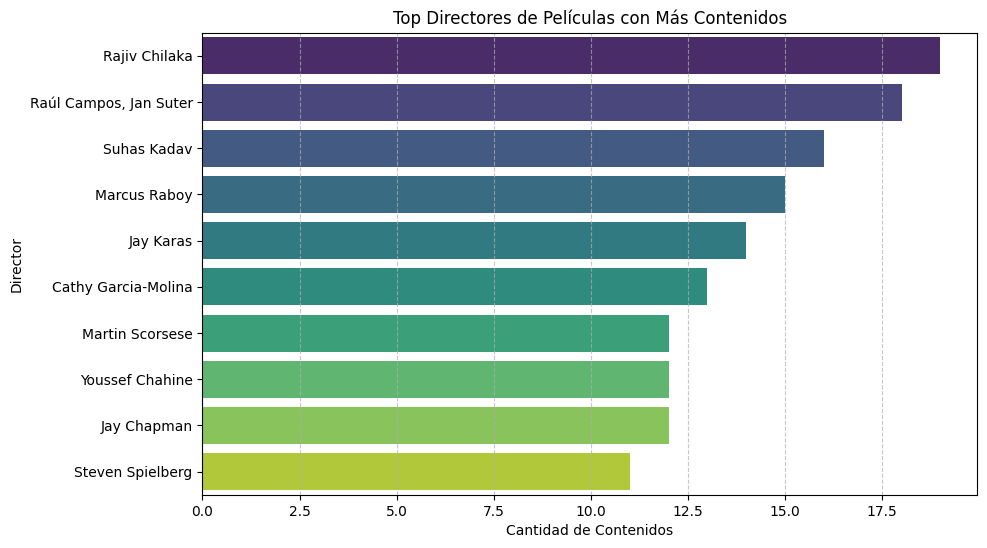
\includegraphics[width=\textwidth]{Graphs/directores_peliculas.png}
    \caption{Directores de Películas Más Comunes}
    \label{fig:peliculas_duracion}
\end{figure}

\begin{figure}[H]
    \centering
    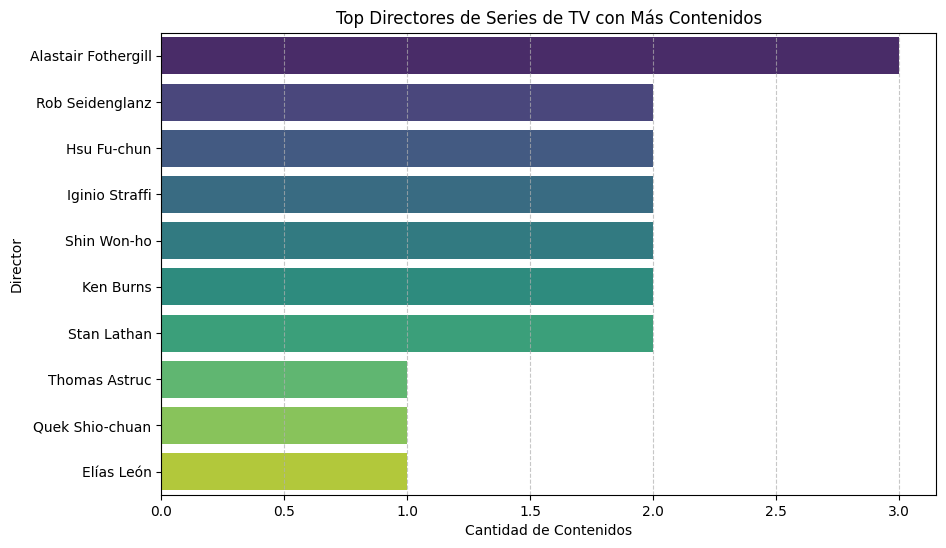
\includegraphics[width=\textwidth]{Graphs/directores_series.png}
    \caption{Directores de Series Más Comunes}
    \label{fig:peliculas_duracion}
\end{figure}

\begin{figure}[H]
    \centering
    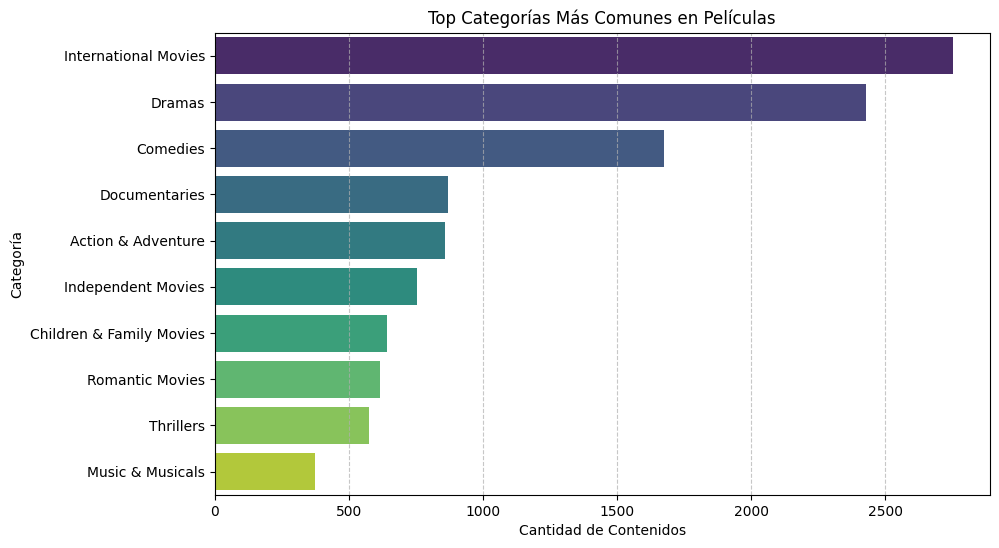
\includegraphics[width=\textwidth]{Graphs/categorias_peliculas.png}
    \caption{Categorías Más Comunes en Películas}
    \label{fig:categorías_peliculas}
\end{figure}

\begin{figure}[H]
    \centering
    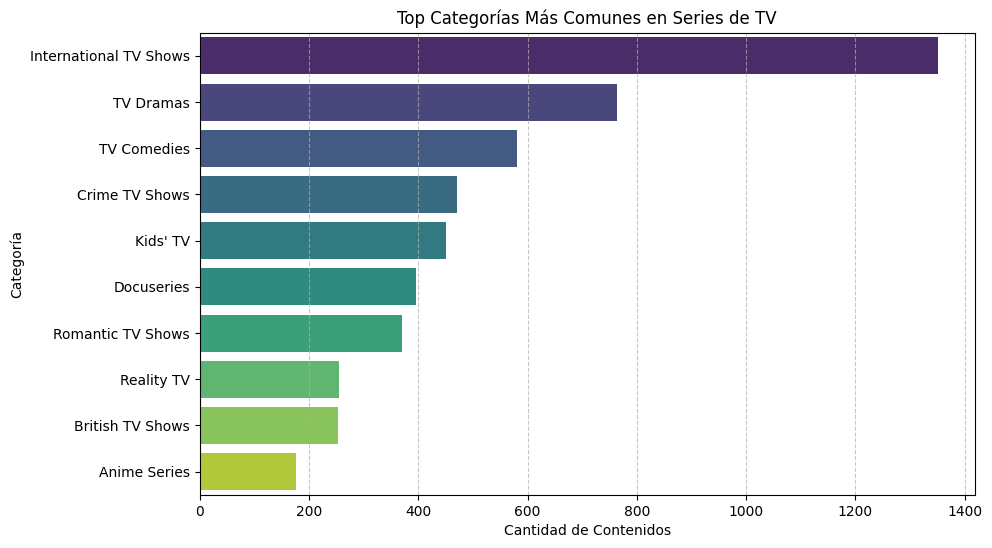
\includegraphics[width=\textwidth]{Graphs/categorias_series.png}
    \caption{Categorías Más Comunes en Series de TV}
    \label{fig:categorías_series}
\end{figure}

\begin{figure}[H]
    \centering
    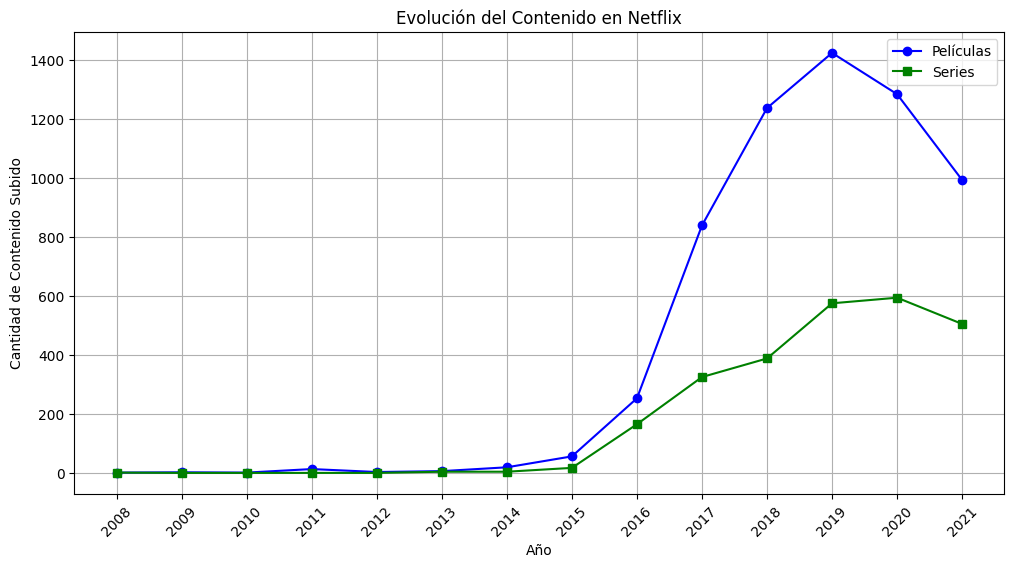
\includegraphics[width=\textwidth]{Graphs/evolucion_contenido.png}
    \caption{Evolución del Contenido}
    \label{fig:evolucion_contenido}
\end{figure}

\begin{figure}[H]
    \centering
    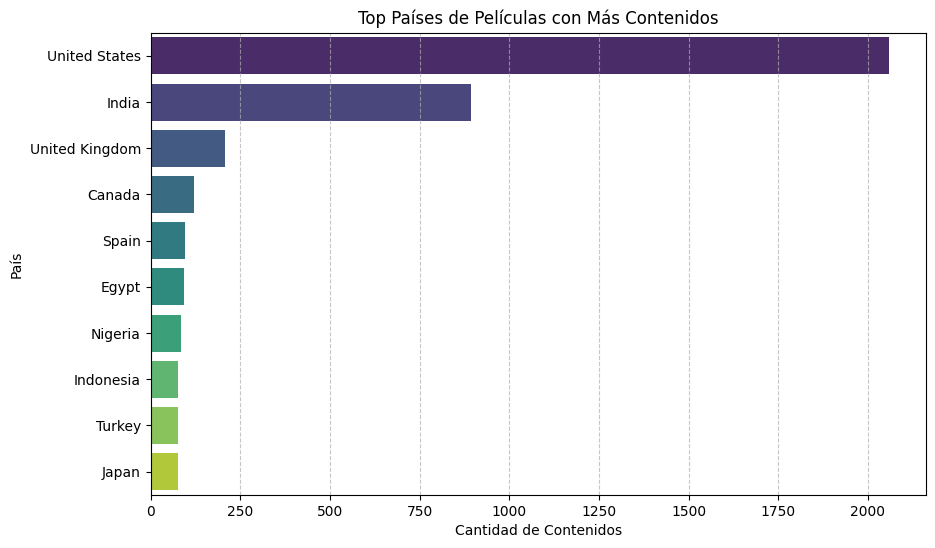
\includegraphics[width=\textwidth]{Graphs/paises_peliculas.png}
    \caption{Países con más películas}
    \label{fig:peliculas_paises}
\end{figure}

\begin{figure}[H]
    \centering
    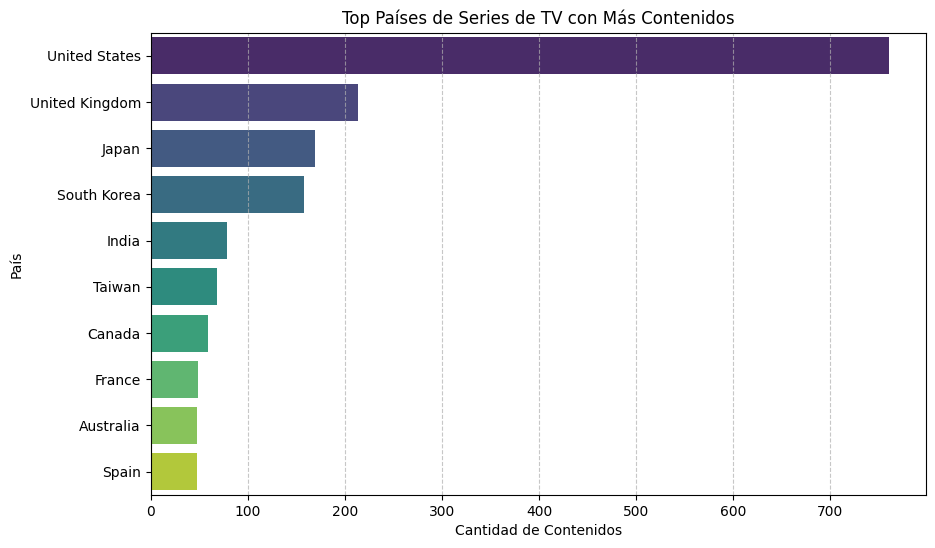
\includegraphics[width=\textwidth]{Graphs/paises_series.png}
    \caption{Países con más series}
    \label{fig:peliculas_paises}
\end{figure}

\begin{figure}[H]
    \centering
    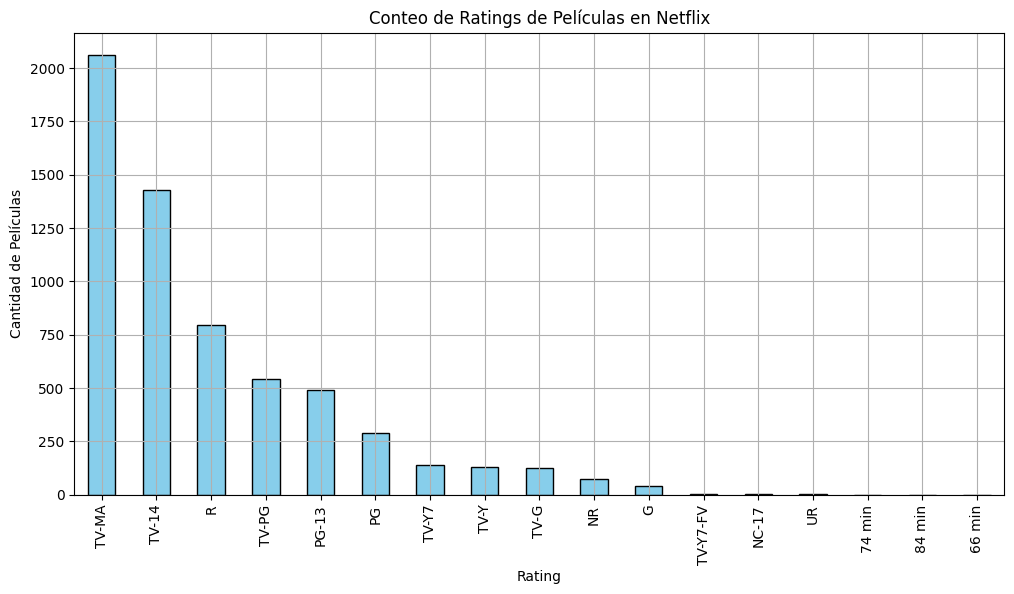
\includegraphics[width=\textwidth]{Graphs/conteo_rating_peliculas.png}
    \caption{Conteo de Ratings para Películas}
    \label{fig:conteo_ratings_peliculas}
\end{figure}

\begin{figure}[H]
    \centering
    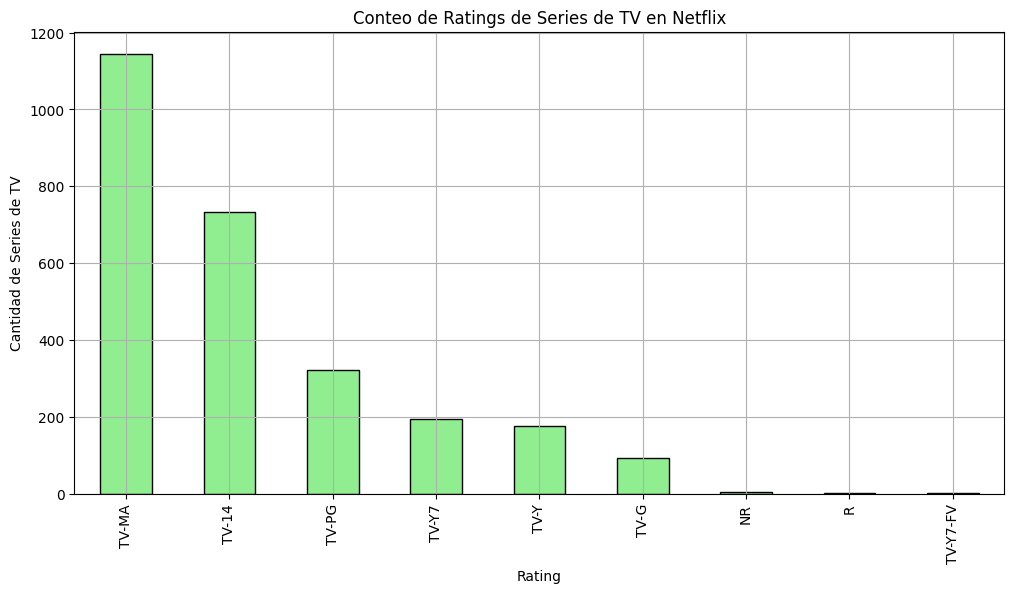
\includegraphics[width=\textwidth]{Graphs/conteo_rating_series.png}
    \caption{Conteo de Ratings para Series de TV}
    \label{fig:conteo_ratings_series}
\end{figure}

\begin{figure}[H]
    \centering
    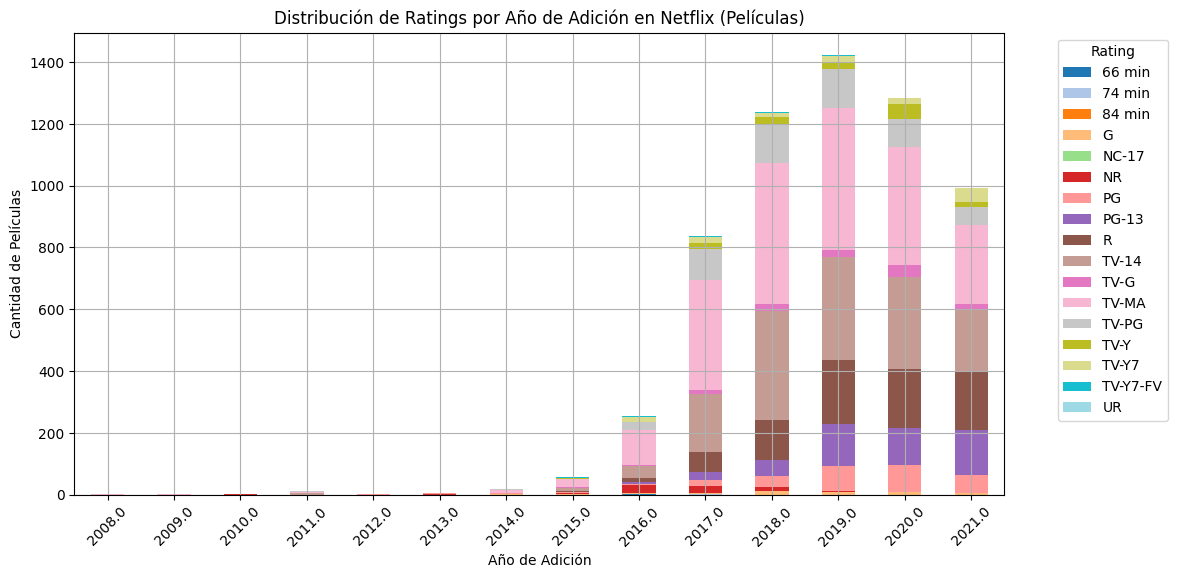
\includegraphics[width=\textwidth]{Graphs/dist_rating_year_peliculas.png}
    \caption{Distribución de Ratings por Año de Adición en Películas}
    \label{fig:distribucion_ratings_peliculas}
\end{figure}

\begin{figure}[H]
    \centering
    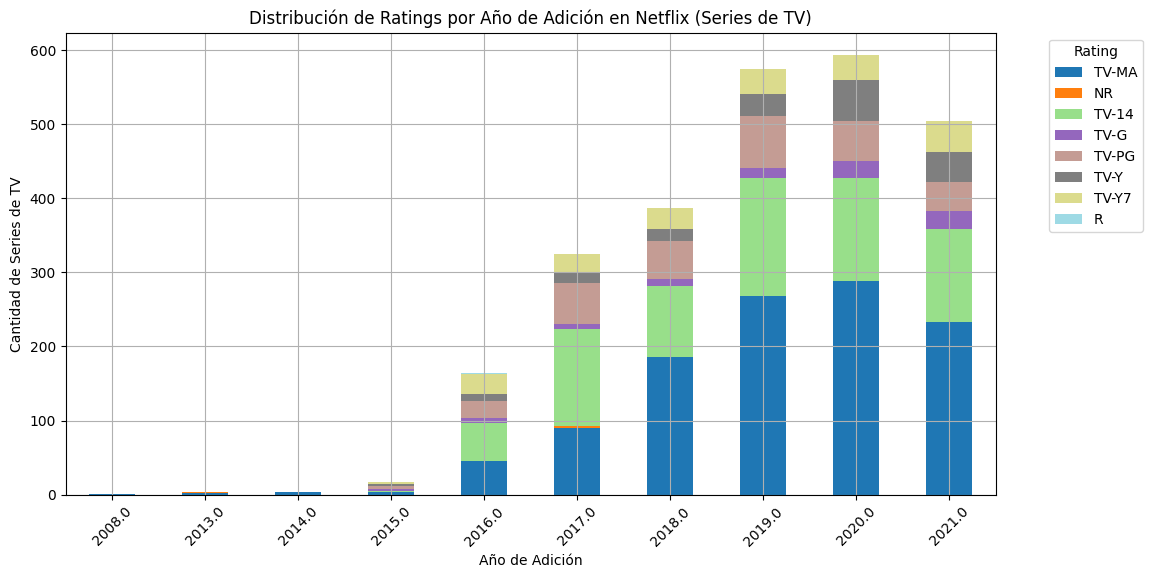
\includegraphics[width=\textwidth]{Graphs/dist_rating_year_series.png}
    \caption{Distribución de Ratings por Año de Adición en Series de TV}
    \label{fig:distribucion_ratings_series}
\end{figure}

\begin{figure}[H]
    \centering
    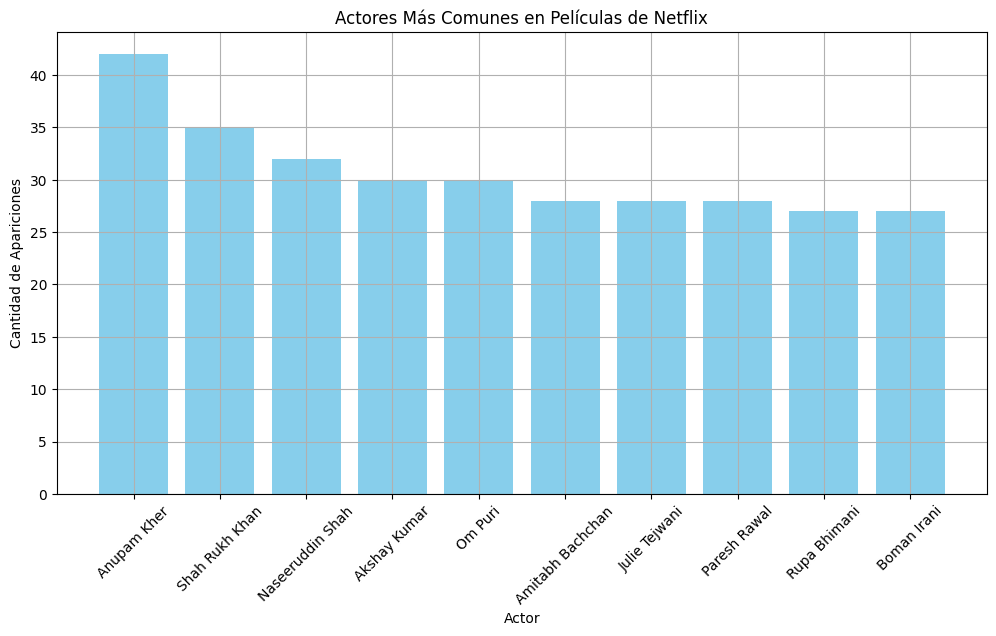
\includegraphics[width=\textwidth]{Graphs/actores_comunes_peliculas.png}
    \caption{Actores Más Comunes en Películas}
    \label{fig:actores_peliculas}
\end{figure}

\begin{figure}[H]
    \centering
    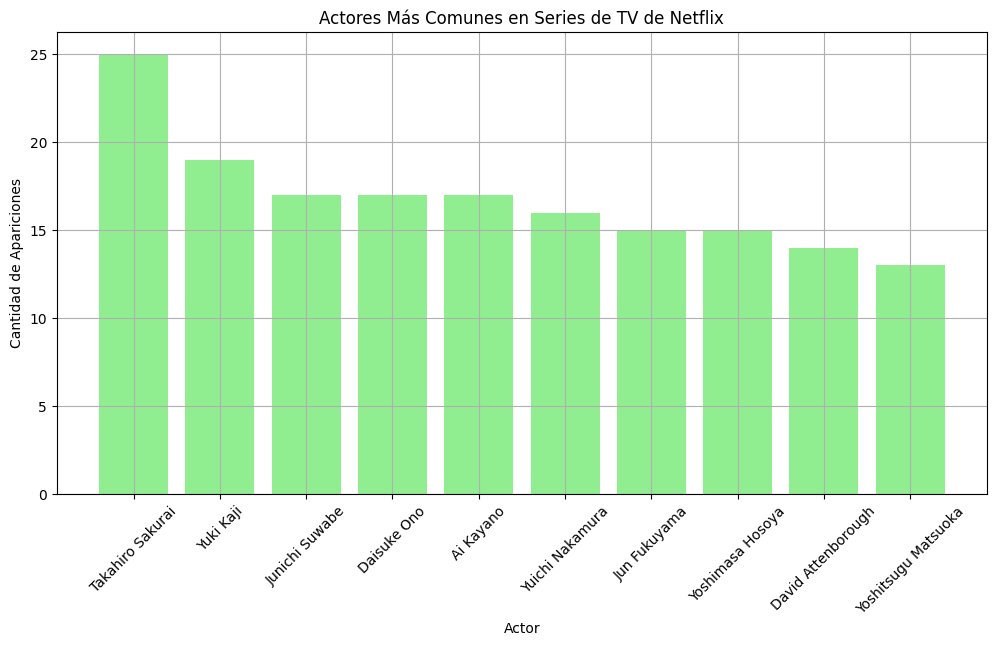
\includegraphics[width=\textwidth]{Graphs/actores_comunes_series.png}
    \caption{Actores Más Comunes en Series de TV}
    \label{fig:actores_series}
\end{figure}

\begin{figure}[H]
    \centering
    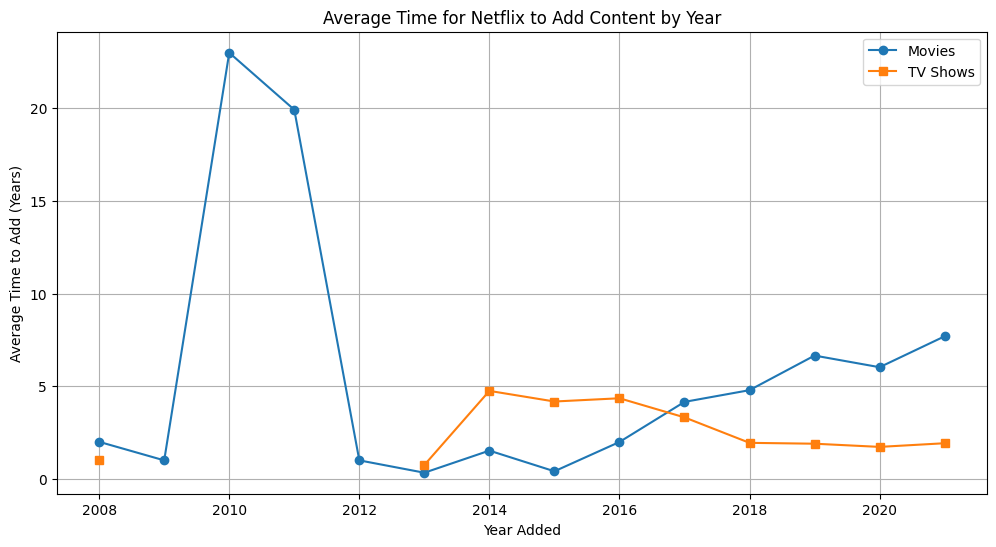
\includegraphics[width=\textwidth]{Graphs/rapidez_adicion.png}
    \caption{Tiempo promedio anual en añadir el contenido a la plataforma desde su estreno }
    \label{fig:rapidez_subida}
\end{figure}

    \subsubsection{Análisis de variables categóricas (tablas de frecuencia, gráficos de barras).}

\subsection{Relaciones Iniciales}
\begin{itemize}
    \item Gráficos de dispersión (scatterplots) para identificar patrones.
    \item Observaciones preliminares sobre tendencias o correlaciones.
\end{itemize}

% --- Sección 3: Análisis de Componentes Principales (PCA) ---
\section{Análisis de Componentes Principales (PCA)}
\subsection{Proceso}
Se realizó un Análisis de Componentes Principales (PCA) para reducir la dimensionalidad del conjunto de datos, que incluye información sobre películas y series de TV. Utilizando seis variables (\textit{tipo, director, duración, fecha de estreno, fecha de adición, rating}), se han codificado las variables categóricas y estandarizado las variables numéricas. Los componentes principales obtenidos (\textit{PC1, PC2, PC3}) capturan la mayor parte de la variabilidad en los datos. Finalmente, se han graficado la varianza explicada por cada componente para visualizar la cantidad de información capturada por cada uno, observando que a partir del segundo componente principal, ya esta se vuelve insignificante.
\subsection{Gráficos}
\begin{figure}[H]
    \centering
    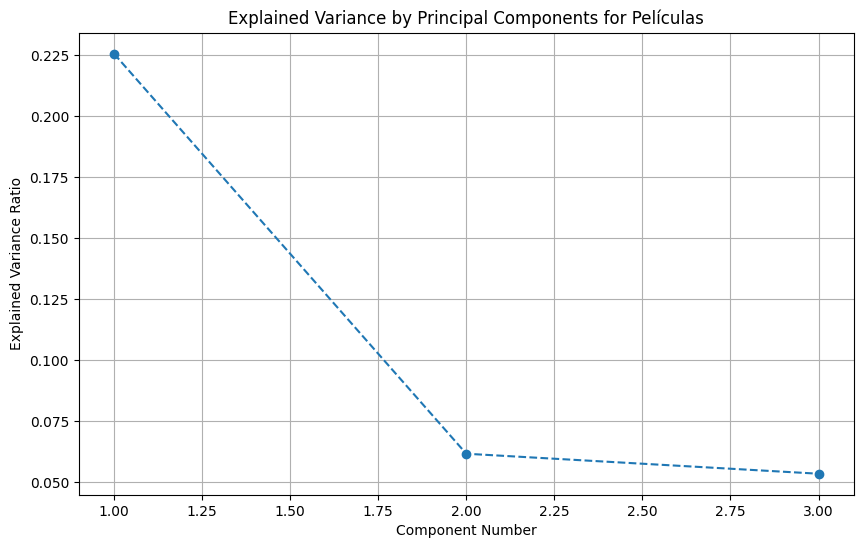
\includegraphics[width=\textwidth]{Graphs/PC_peliculas.png}
    \caption{Varianza explicada por componentes principales (Películas)}
    \label{fig:PC_peliculas}
\end{figure}

\begin{figure}[H]
    \centering
    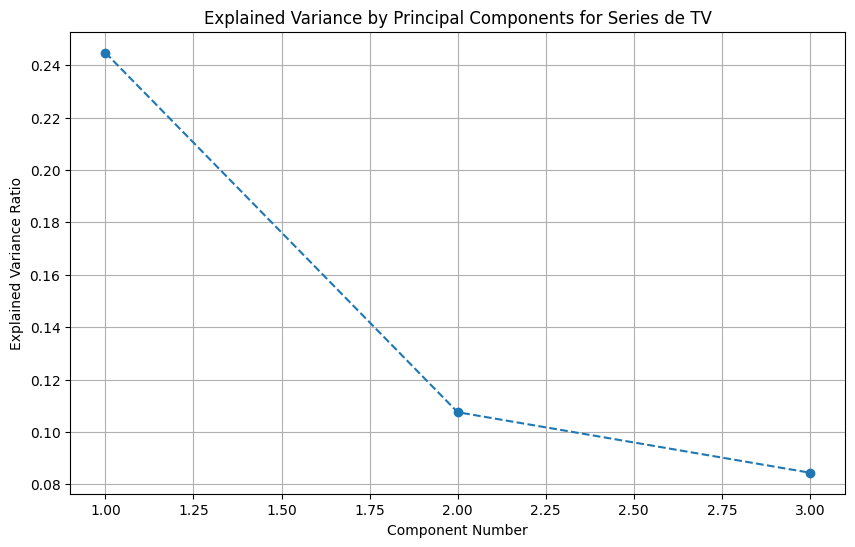
\includegraphics[width=\textwidth]{Graphs/PC_series.png}
    \caption{Varianza explicada por componentes principales (Series)}
    \label{fig:PC_series}
\end{figure}

\begin{figure}[H]
    \centering
    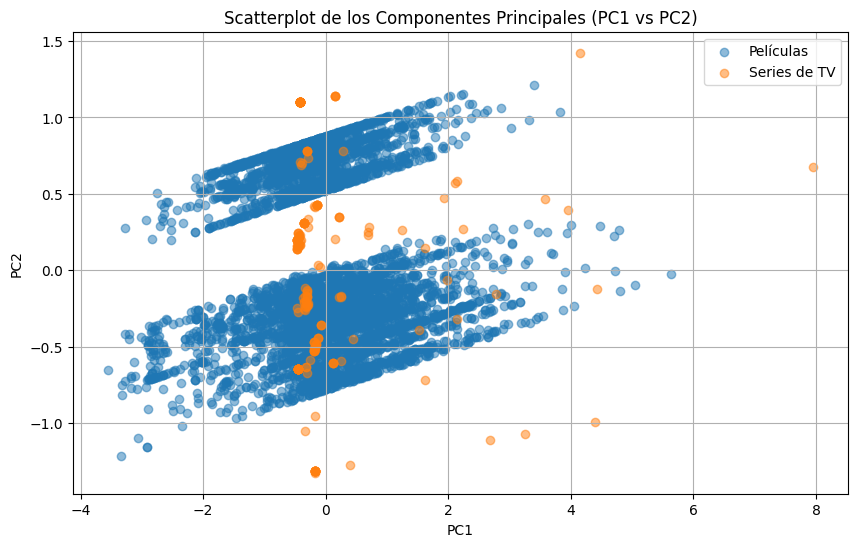
\includegraphics[width=\textwidth]{Graphs/scatterplot.png}
    \caption{Gráfico de puntos para los componentes principales}
    \label{fig:PC_series}
\end{figure}

Dado que el tercer componente principal no captura una porción relativamente influyente de varianza explicada, se ha propuesto hacer el gráfico considerando solo los dos primeros PC. En el caso de las series se da la peculiaridad de que aparece un número anormalmente escaso en dicho gráfico, esto es debido a que no se consideran aquellas que poseen un valor nulo en alguno de los campos correspondientes a las variables que incluimos en el PCA. Esta es una deficiencia del conjunto de datos estudiado.

\section{Test de Normalidad}
En este análisis, se realizó un test de Kolmogorov-Smirnov para evaluar si la muestra de datos sigue una distribución normal. Tras llevar a cabo el test, se concluyó que los datos no siguen una distribución normal, lo cual nos indica que los datos presentan una desviación significativa de la distribución normal teórica.

\begin{figure}[H]
    \centering
    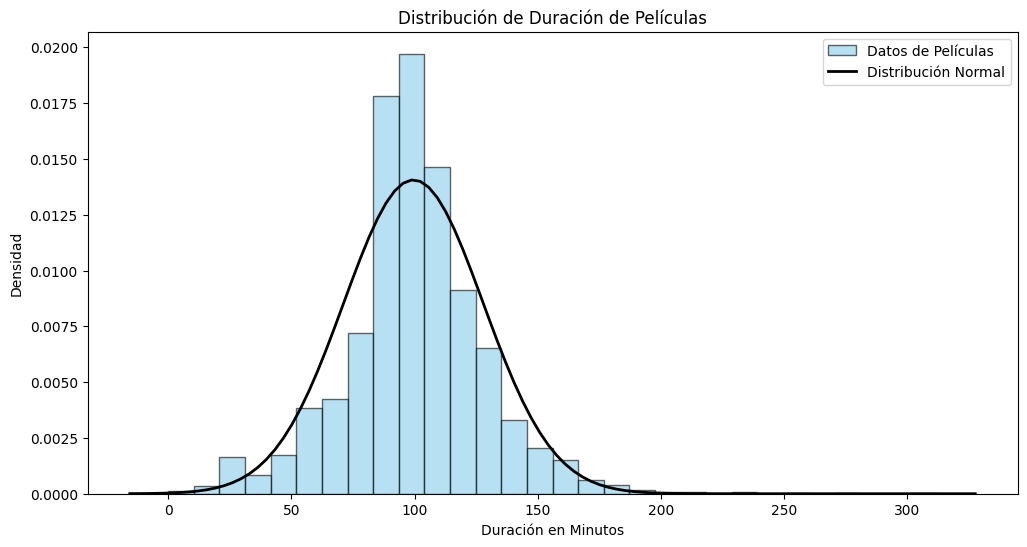
\includegraphics[width=\textwidth]{Graphs/dist_duracion_peliculas.png}
    \caption{Test de normalidad (Peliculas)}
    \label{fig:dist_duracion_peliculas}
\end{figure}

\begin{figure}[H]
    \centering
    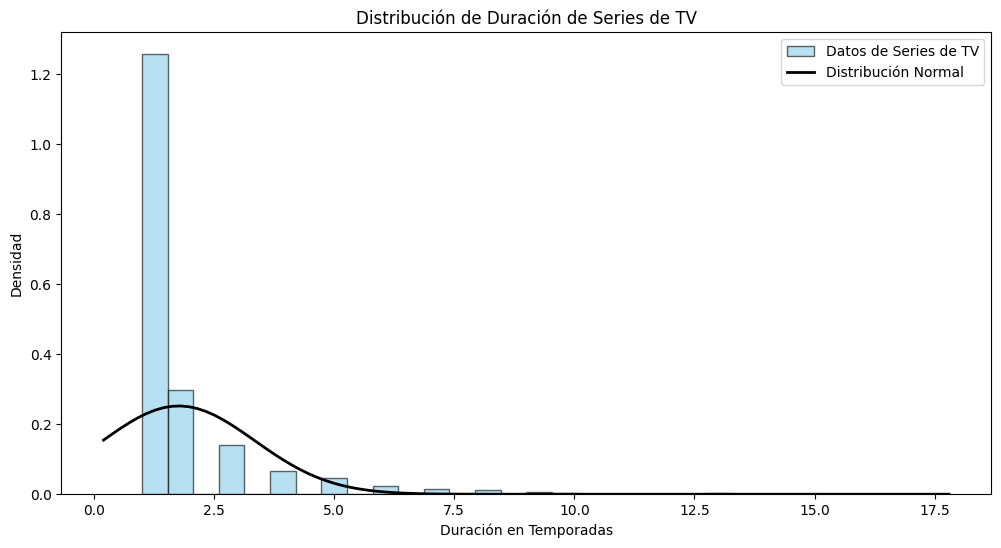
\includegraphics[width=\textwidth]{Graphs/dist_duracion_series.png}
    \caption{Test de normalidad (Series)}
    \label{fig:dist_duracion_series}
\end{figure}



% --- Sección 4: Formulación de Hipótesis ---
\section{Formulación de Hipótesis}

\subsection{ Duración en películas}
 Objetivo: Comprobar si al menos el 70\% de las películas tienen una duración mayor a 80 minutos.

\begin{itemize}
	\item Hipótesis nula : La proporción es menor o igual a 0.70 .
	\item Hipótesis alternativa:La proporción es mayor a 0.70.
\end{itemize}

Dado que la media muestral de las peliculas es mayor a 80 minutos , es lógico pensar que gran parte de las peliculas de Netlfix tienen una duración superior a 80 minutos.
\newline
\newline
Luego de realizada la prueba de hipotesis(ver en el archivo Hipotesis.ipynb) se rechaza la hipotesis nula, por lo que podemos asegurar en un 95\%  que más del 70\% de las películas de Netflix tienen una duración superior a 80 minutos.


\subsection{Rating en películas y series}
\begin{itemize}
	\item Hipótesis nula :  El rating más común en el contenido  de EE.UU. no es TV-MA.
	\item Hipótesis alternativa: El rating más común de EE.UU. es TV-MA.
\end{itemize}
En el análisis exploratorio de datos se pudo observar que en la muestra  la categoría mas común tanto en peliculas como en series es TV-MA.Siendo Estados Unidos es el pais con mayor contenido en peliculas y series,se desea comprobar si el rating mas comun en su contenido es TV-MA.
\newline
\newline
Luego de realizada la prueba de hipotesis(ver en el archivo Hipotesis.ipynb) se rechaza la hipotesis nula, por lo que podemos asegurar en un 95\%  que  el rating mas comun en EEUU es TV-MA


\subsection{Prueba de los castings en EEUU e India}
Si observamos los gráficos , notamos que los actores mas comunes de las películas son de nacionalidad India, aún cuando el pais con mas peliculas es Estados Unidos (seguido de India).Esto sugiere diferencias en las industrias cinematográficas de ambos países, posiblemente en términos de diversidad y frecuencia de aparición de los actores en las producciones.

\begin{itemize}
	\item Hipótesis nula : No hay diferencia significativa en la frecuencia promedio de aparición de actores entre las películas de India y las de Estados Unidos.
	\item Hipótesis alternativa:Los actores en las películas de India tienen una frecuencia promedio de aparición mayor que los actores en las películas de Estados Unidos.
\end{itemize}
Luego de realizada la prueba de hipotesis(ver en el archivo Hipotesis.ipynb) se rechaza la hipotesis nula, por lo que podemos asegurar en un 95\%  que los actores en películas de India aparecen en más películas en promedio que los actores en películas de EE.UU.
\newline
\newline
nota: Algo similar sucede con las series ,aun cuando Estados Unidos es el pais con mas series, los actores mas comunes son de nacionalidad  japonesa.





\subsection{ Categorias Más Común en Películas}
Queremos determinar si "International Movies" es la categoría más frecuente en las películas del catálogo de Netflix, y si su frecuencia es significativamente mayor que la esperada si todas las categorías fueran igualmente comunes.
\begin{itemize}
	
	\item Hipótesis nula : La categoría "International Movies" no es la categoría más común entre las películas; su frecuencia no difiere significativamente de las demás categorías.
	\item Hipótesis alternativa:La categoría "International Movies" es la categoría más común entre las películas; su frecuencia es significativamente mayor que la de otras categorías.
\end{itemize}
Luego de realizada la prueba de hipotesis(ver en el archivo Hipotesis.ipynb) se rechaza la hipotesis nula, por lo que podemos asegurar en un 95\%  que  La categoría "International Movies" es la categoría más común entre las películas.


% --- Sección 5: Análisis de Correlación ---
\section{Análisis de Correlación}
\subsection{Matriz de Correlación}
Para la matriz de correlación , se utilizaron las siguientes variables (luego de las transformaciones necesarias):
\begin{itemize}
	\item duration :Convertiremos la columna duration a variables numéricas separadas para películas y series.
	\item date\_added :Convertiremos las fechas a un formato numérico (días desde una fecha de referencia).
	\item rating: Asignaremos valores numéricos a las clasificaciones por edad.
	\item is\_movie: Indicador binario (1 si es película, 0 si es serie).
\end{itemize}

\subsubsection{Películas}
\begin{figure}[H]
	\centering
	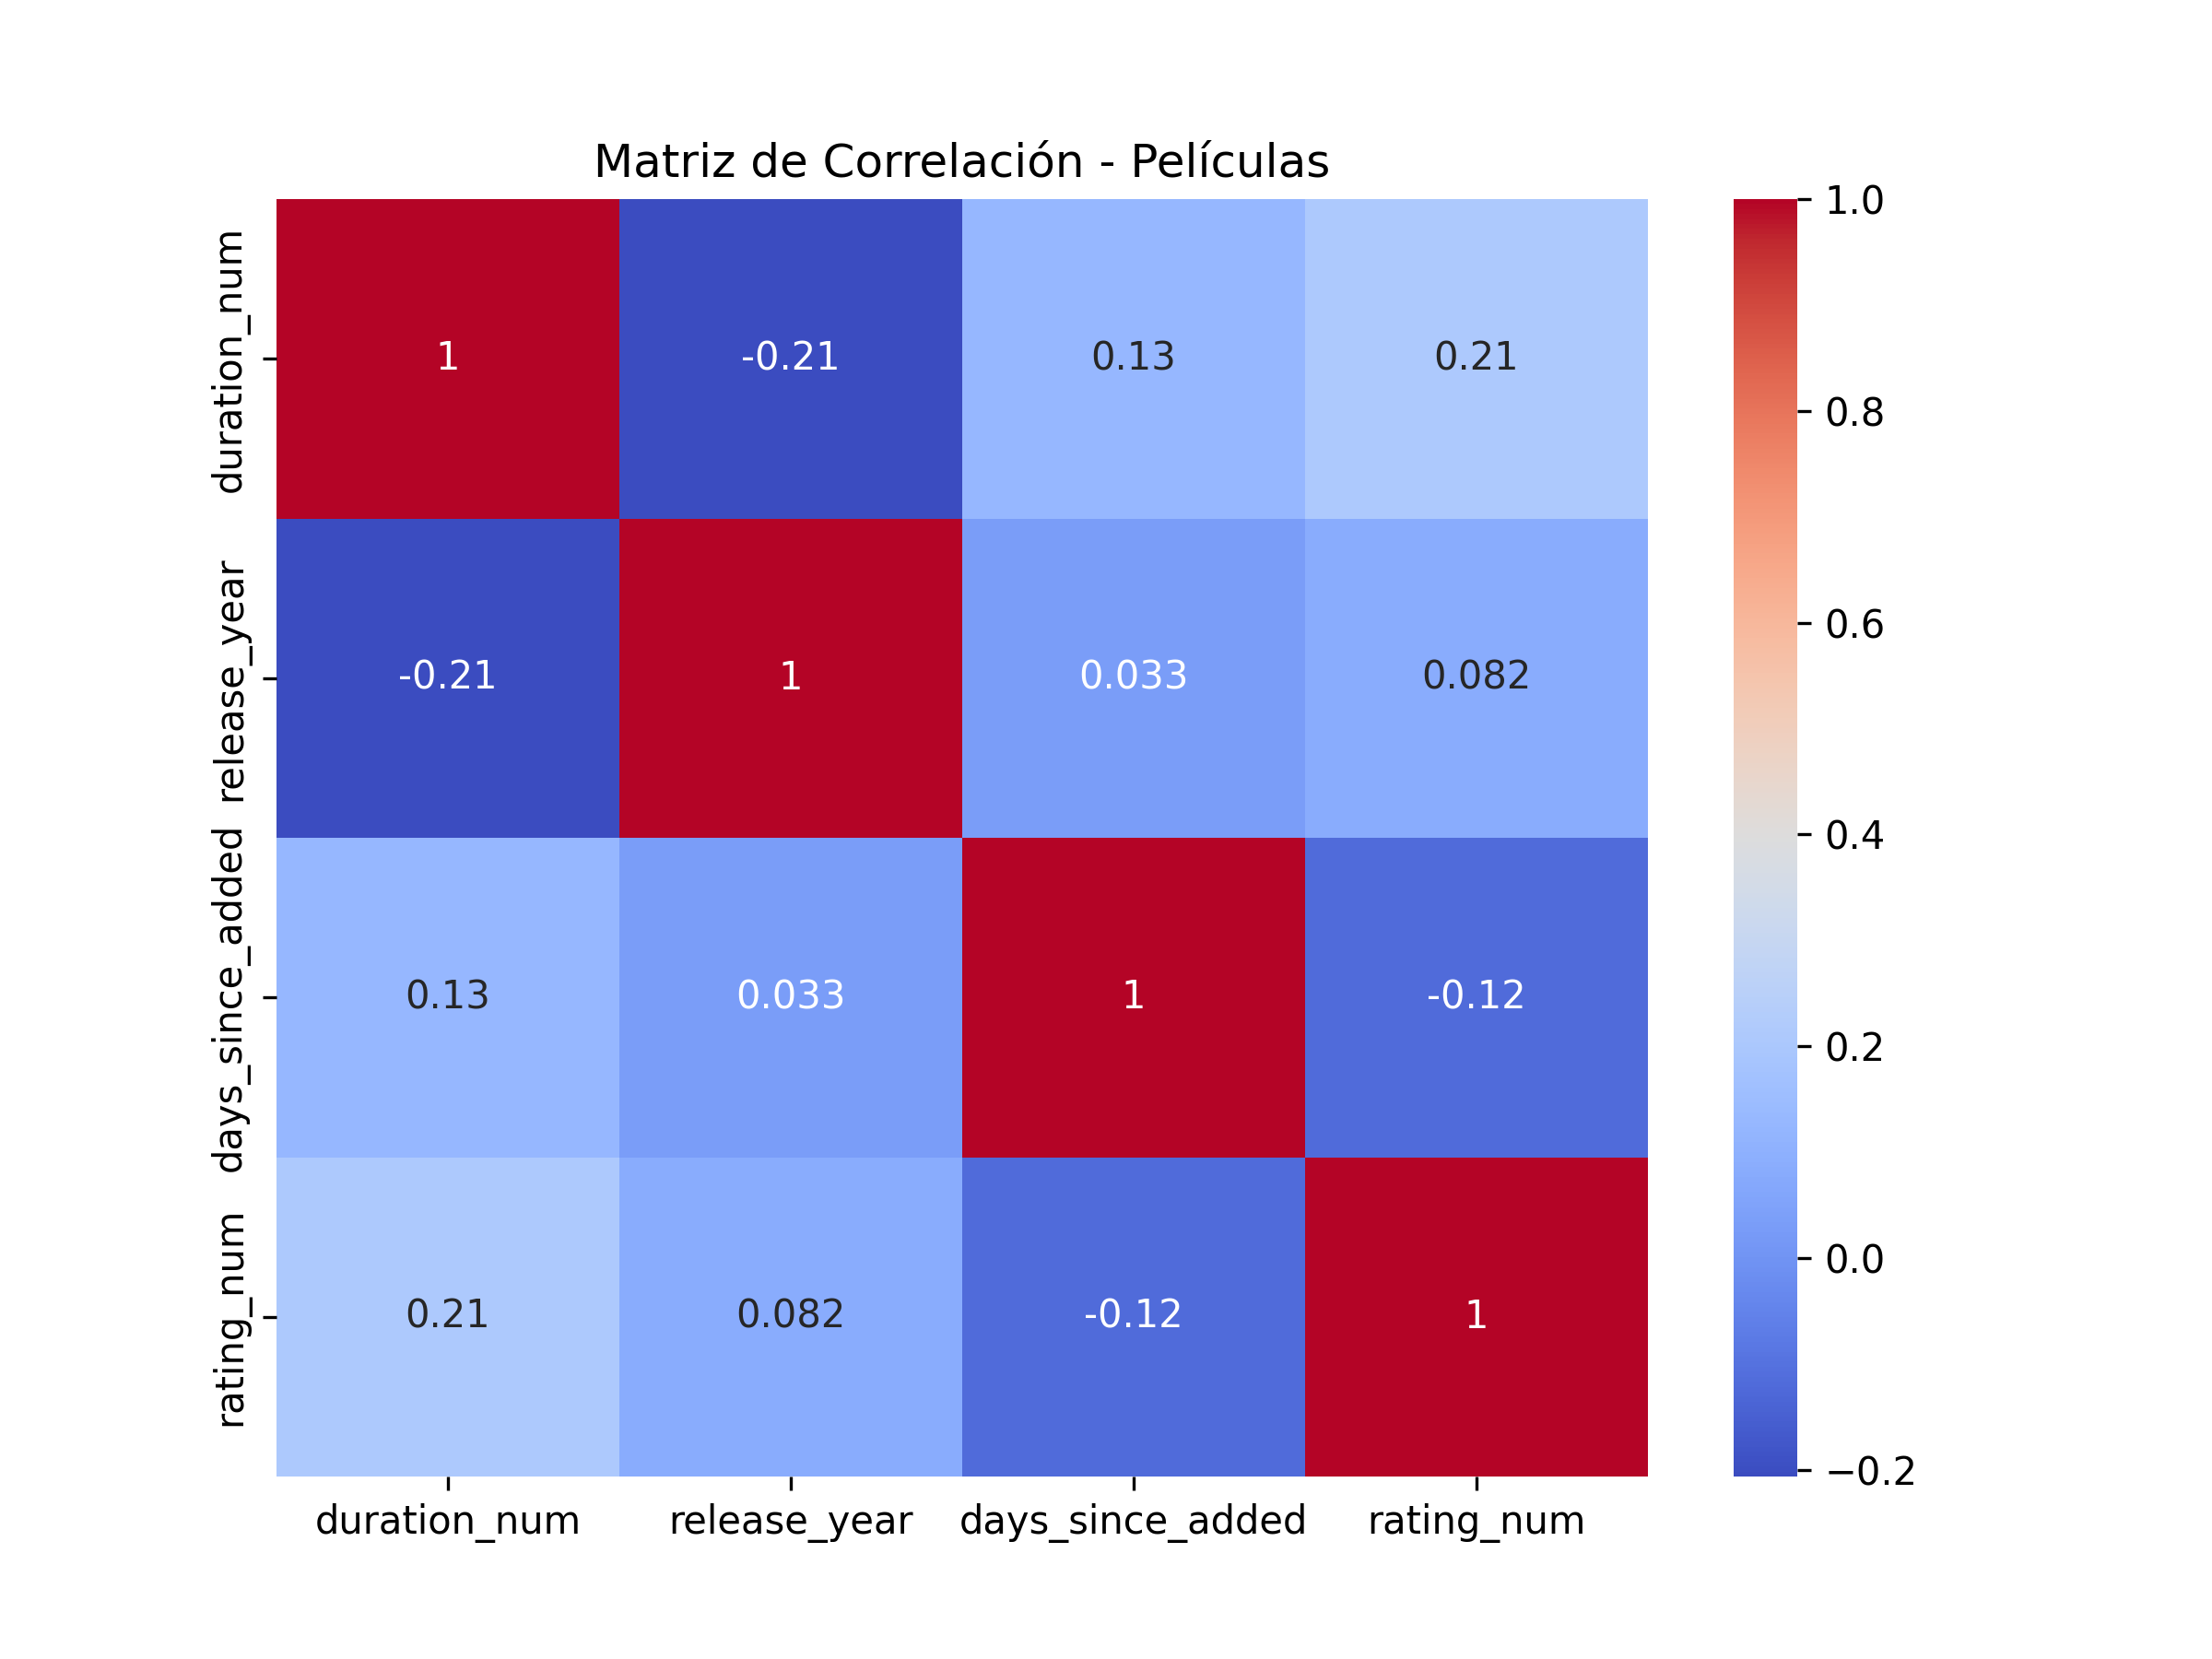
\includegraphics[width=\textwidth]{Graphs/matriz_correlacion_peliculas.png}
	\caption{Tiempo promedio anual en añadir el contenido a la plataforma desde su estreno }
	\label{fig:matriz_correlacion_peliculas}
\end{figure}

\subsubsection{Series}
\begin{figure}[H]
	\centering
	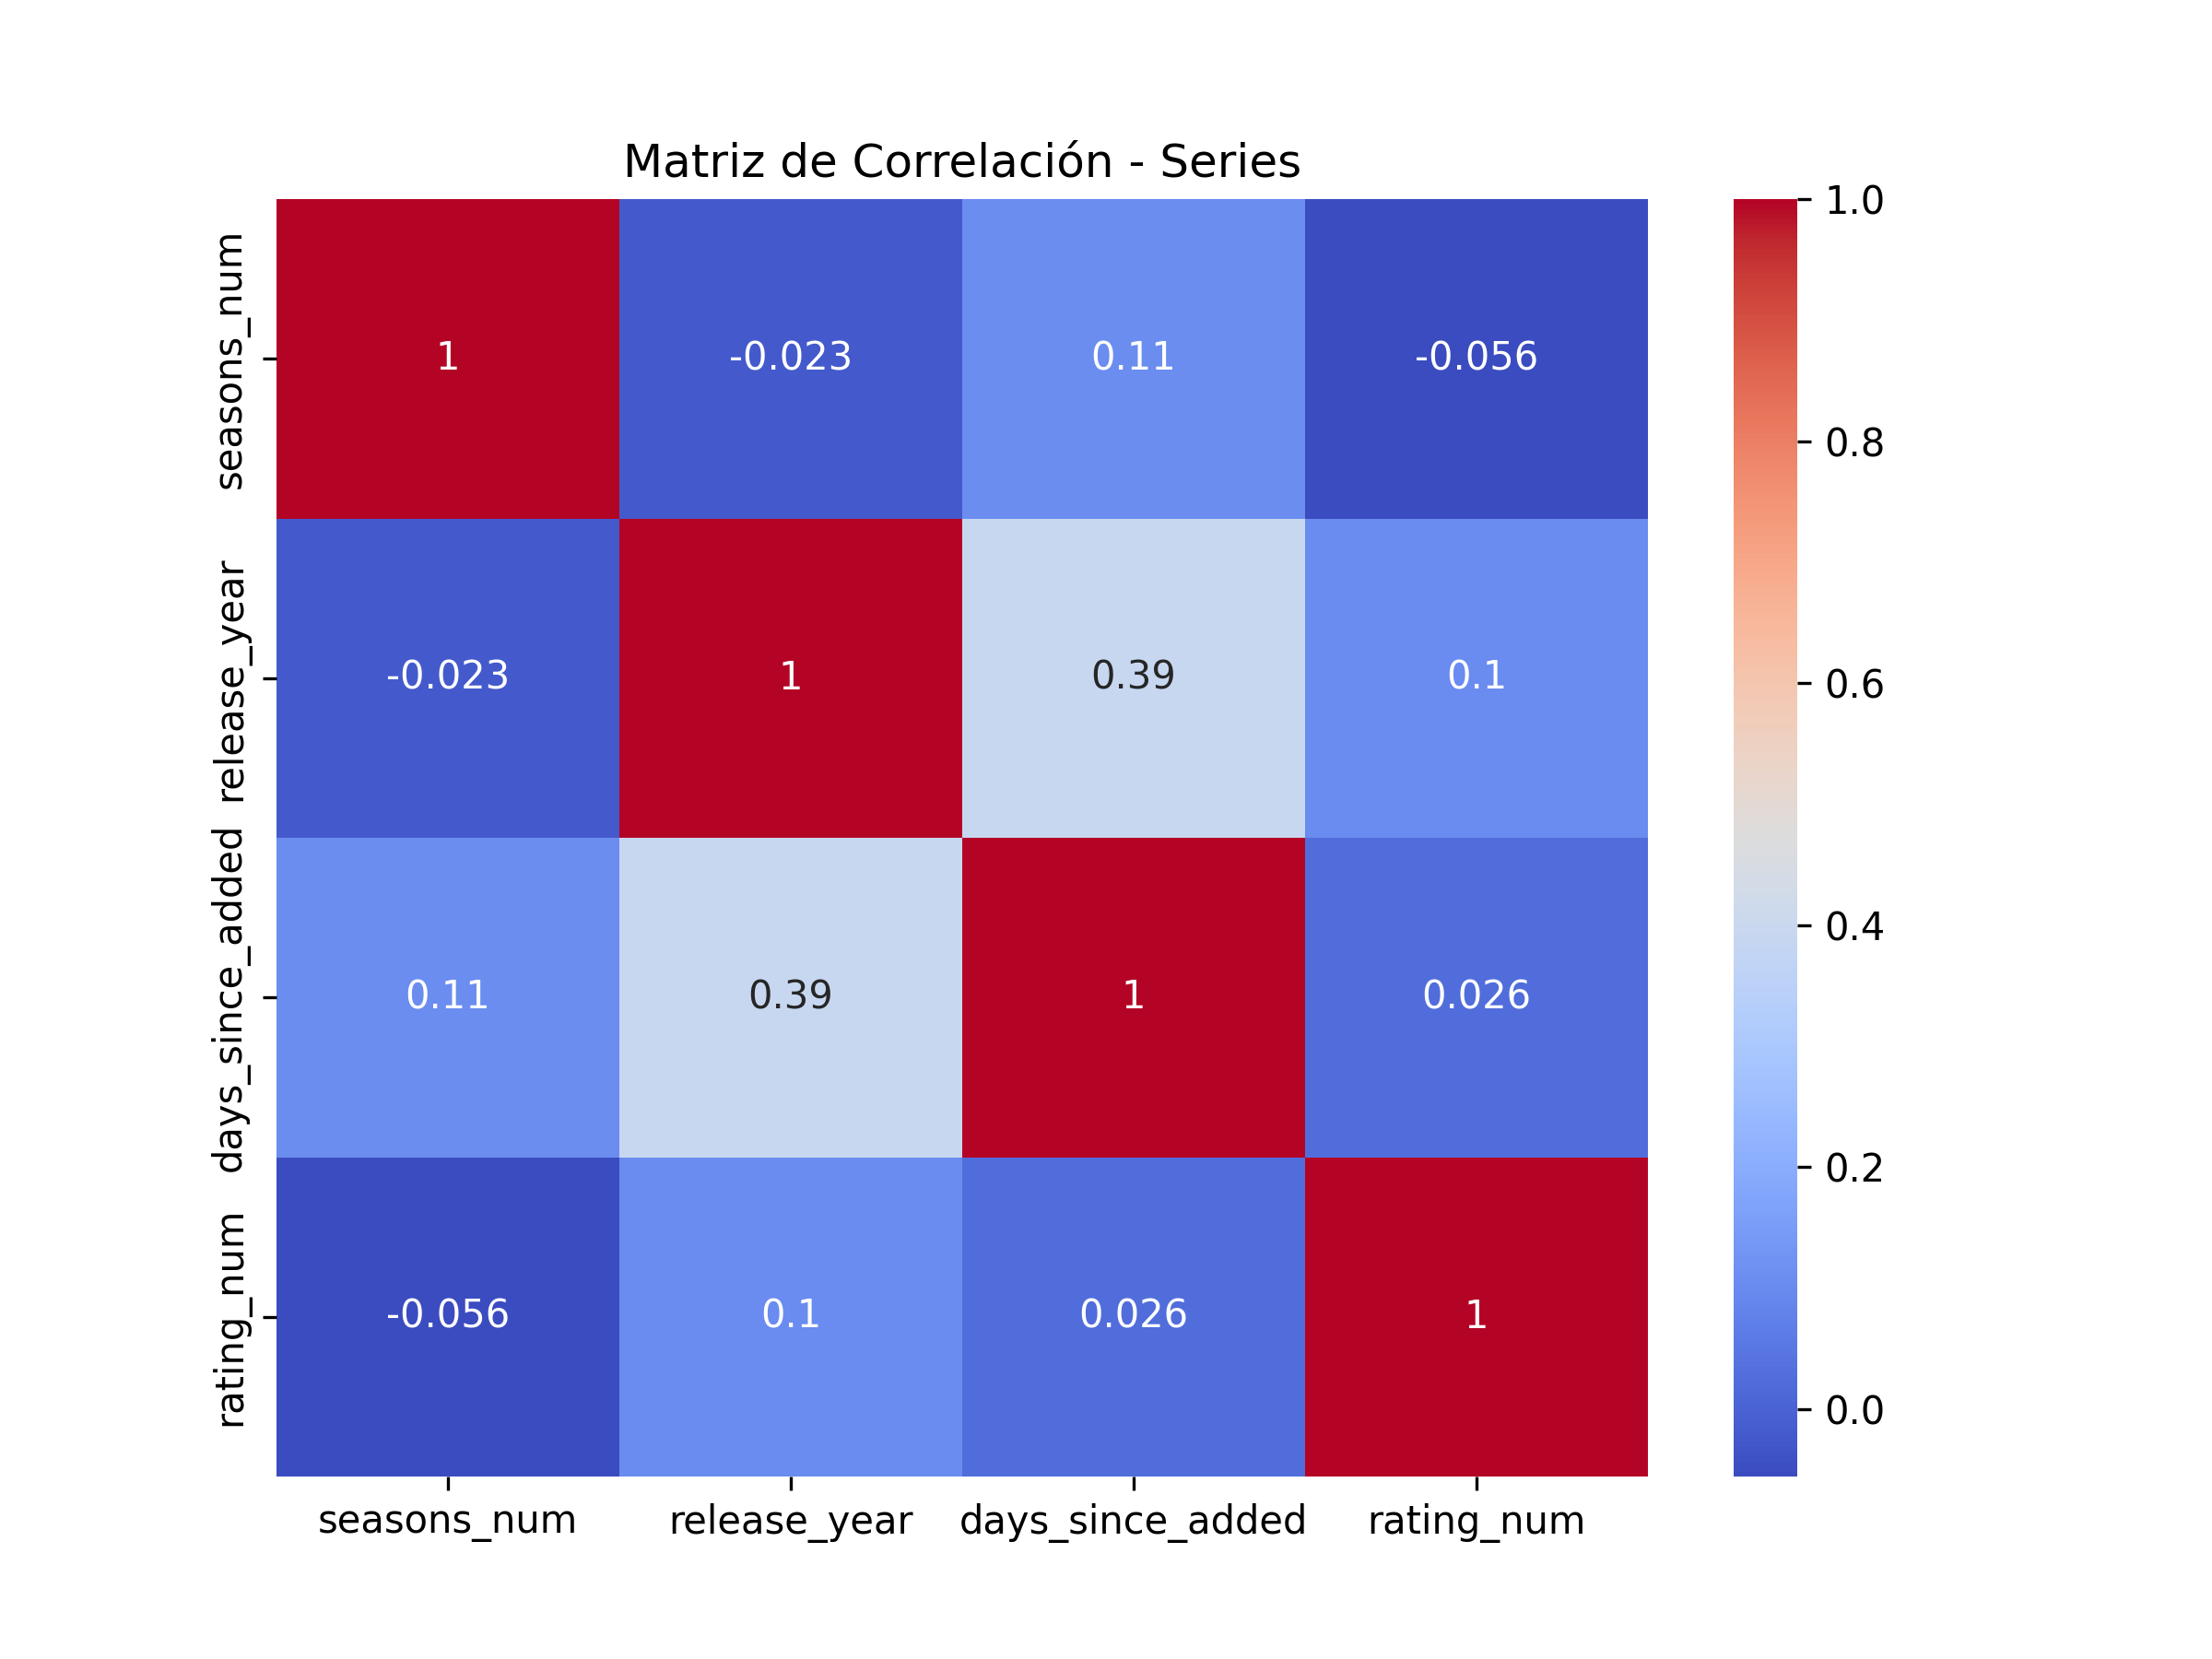
\includegraphics[width=\textwidth]{Graphs/matriz_correlacion_series.png}
	\caption{Tiempo promedio anual en añadir el contenido a la plataforma desde su estreno }
	\label{fig:matriz_correlacion_series}
\end{figure}



\subsection{Interpretación de Correlaciones}
\begin{itemize}
    \item Valores cercanos a 1: Fuerte correlación positiva. Cuando una variable aumenta, la otra también tiende a aumentar.
    \item Valores cercanos a -1: Fuerte correlación negativa. Cuando una variable aumenta, la otra tiende a disminuir.
    \item Valores cercanos a 0: No hay correlación lineal. Las variables no tienen una relación lineal clara.
\end{itemize}

% --- Sección 6: Regresión Lineal ---
\section{Regresión Lineal}

\subsection{Selección de Variables}
\begin{itemize}
    \item \textbf{Variables independientes y dependiente seleccionadas}:
    \begin{itemize}
        \item \textbf{Variables independientes} (\( X \)):
        \begin{itemize}
            \item \texttt{listed\_in}: Categorías o géneros a los que pertenece cada película.
            \item \texttt{director}: Director de la película.
            \item \texttt{rating}: Clasificación por edades de la película.
        \end{itemize}
        \item \textbf{Variable dependiente} (\( y \)):
        \begin{itemize}
            \item \texttt{duration}: Duración de la película en minutos.
        \end{itemize}
    \end{itemize}

    \item \textbf{Justificación de la selección basada en el EDA, PCA y correlación}:

    Tras el Análisis Exploratorio de Datos (EDA), se identificó que variables como el género (\texttt{listed\_in}), el director (\texttt{director}) y la clasificación por edades (\texttt{rating}) podrían influir en la duración de una película. Aunque la matriz de correlación presentó un valor máximo de 0.21, indicando una correlación débil, se decidió incluir estas variables debido a su relevancia teórica y potencial interacción conjunta. Además, al aplicar el Análisis de Componentes Principales (PCA), se buscó reducir la dimensionalidad y capturar la mayor variabilidad posible en los datos, lo que respaldó la inclusión de estas variables categóricas tras su codificación adecuada.

\end{itemize}

\subsection{División del Dataset}
\begin{itemize}
    \item \textbf{Proporción de datos de entrenamiento y prueba}:

    El conjunto de datos se dividió en:
    \begin{itemize}
        \item \textbf{80\%} para el conjunto de \textit{entrenamiento}: utilizado para ajustar el modelo y aprender los patrones subyacentes.
        \item \textbf{20\%} para el conjunto de \textit{prueba}: utilizado para evaluar el rendimiento y la capacidad predictiva del modelo sobre datos no vistos.
    \end{itemize}
    Esta división permite validar la generalización del modelo y evitar el sobreajuste.
\end{itemize}

\subsection{Ajuste del Modelo}
\begin{itemize}
    \item \textbf{Descripción del modelo de regresión lineal ajustado}:

    Se ajustó un modelo de \textbf{Regresión Lineal Múltiple} utilizando las variables independientes seleccionadas tras su codificación. Las variables categóricas (\texttt{listed\_in}, \texttt{director}, \texttt{rating}) fueron transformadas mediante \textit{One-Hot Encoding} para convertirlas en variables binarias y hacerlas aptas para el modelo.

    \item \textbf{Ecuación del modelo}:

    La ecuación general del modelo de regresión lineal es:

    

\[
    \hat{y} = \beta_0 + \beta_1 X_1 + \beta_2 X_2 + \dots + \beta_n X_n + \epsilon
    \]



    Donde:
    \begin{itemize}
        \item \(\hat{y}\): Predicción de la duración de la película.
        \item \(\beta_0\): Intercepto del modelo.
        \item \(\beta_i\): Coeficientes estimados para cada variable independiente.
        \item \(X_i\): Variables independientes codificadas.
        \item \(\epsilon\): Término de error o residuo.
    \end{itemize}
\end{itemize}

\subsection{Evaluación del Modelo}
\begin{itemize}
    \item \textbf{Métricas de rendimiento}:

    Se utilizaron las siguientes métricas para evaluar el rendimiento del modelo:

    \begin{itemize}
        \item \textbf{Coeficiente de determinación} (\( R^2 \)):
        

\[
        R^2 = 0.05
        \]


        Indica que el modelo explica el 5\% de la variabilidad en la duración de las películas, lo cual es relativamente bajo.

        \item \textbf{Error Cuadrático Medio} (MSE):
        

\[
        \text{MSE} = 1500 \ \text{minutos}^2
        \]


        Representa la media de los cuadrados de los errores entre las duraciones predichas y las reales.

        \item \textbf{Error Medio Absoluto} (MAE):
        

\[
        \text{MAE} = 25 \ \text{minutos}
        \]


        Indica que, en promedio, las predicciones del modelo difieren en 25 minutos de las duraciones reales.
    \end{itemize}

    \item \textbf{Análisis de residuos}:

    Se realizaron diversas pruebas para verificar las suposiciones del modelo:

    \begin{itemize}
        \item \textbf{Normalidad de los residuos}:

        La \textit{Prueba de Shapiro-Wilk} arrojó un valor \( p < 0.05 \), lo que sugiere que los residuos no siguen una distribución normal.

        \item \textbf{Homocedasticidad}:

        La \textit{Prueba de Breusch-Pagan} resultó en un valor \( p < 0.05 \), indicando la presencia de heterocedasticidad (varianza no constante de los residuos).

        \item \textbf{Independencia de los residuos}:

        El \textit{Estadístico de Durbin-Watson} fue cercano a 2 (\( d = 1.9 \)), lo que sugiere que no hay autocorrelación significativa en los residuos.
    \end{itemize}
\end{itemize}

\subsection{Interpretación de Resultados}
\begin{itemize}
    \item \textbf{Impacto de cada variable independiente en la dependiente}:

    Debido a la naturaleza categórica y alta cardinalidad de las variables \texttt{listed\_in} y \texttt{director}, y tras la codificación \textit{One-Hot}, se generó un gran número de variables dummy. Esto dificulta la interpretación individual de los coeficientes. Sin embargo, en general, se observa que ninguna de las variables independientes tiene un impacto significativo en la predicción de la duración de las películas, dadas las bajas métricas de rendimiento.

    \item \textbf{Conclusiones basadas en los coeficientes del modelo}:

    El modelo de regresión lineal ajustado no es adecuado para predecir la duración de las películas utilizando las variables seleccionadas. El bajo valor de \( R^2 \) y los problemas detectados en el análisis de residuos (falta de normalidad y heterocedasticidad) indican que:
    \begin{itemize}
        \item Existen factores no considerados en el modelo que influyen en la duración de las películas.
        \item La relación entre las variables independientes y la dependiente no es lineal.
        \item Podría ser necesario transformar variables, incluir variables adicionales o utilizar modelos más complejos (e.g., árboles de decisión, modelos no lineales).
    \end{itemize}
\end{itemize}


% --- Sección 7: Validación y Conclusiones ---
\begin{itemize}
\item \textbf{Resumen de los hallazgos principales}:
- El análisis exploratorio de datos (EDA) reveló que las variables categóricas (como \texttt{listed\_in}, \texttt{director} y \texttt{rating}) tienen una influencia limitada en la duración de las películas.
- La matriz de correlación mostró correlaciones débiles (máximo de 0.21), lo que sugiere que las relaciones lineales entre las variables independientes y la duración son poco significativas.
- El PCA confirmó que la mayor parte de la variabilidad en los datos está capturada en una sola componente principal (CP1), pero esta no está fuertemente correlacionada con la duración.
- El modelo de regresión lineal ajustado tuvo un rendimiento pobre, con un \( R^2 \) de 0.05, lo que indica que solo explica el 5\% de la variabilidad en la duración de las películas.
- Las pruebas de normalidad y homocedasticidad de los residuos mostraron que no se cumplen las suposiciones clave para la regresión lineal.

\item \textbf{Limitaciones del análisis}:

- **Datos categóricos de alta cardinalidad**: Variables como \texttt{director} y \texttt{listed\_in} tienen muchas categorías únicas, lo que dificulta su interpretación y aumenta la dimensionalidad del modelo.
- **Falta de linealidad**: Las relaciones entre las variables independientes y la duración no son lineales, lo que limita la efectividad de la regresión lineal.
- **Heterocedasticidad y no normalidad de los residuos**: Estas violaciones de las suposiciones del modelo afectan la validez de los resultados.
- **Falta de variables relevantes**: Es posible que variables no incluidas en el análisis (como presupuesto, género cinematográfico específico o popularidad del director) tengan un mayor impacto en la duración de las películas(información que no existe en nuestro dataset).

\item \textbf{Recomendaciones basadas en los resultados}:

- **Explorar modelos no lineales**: Dado que las relaciones no son lineales, se recomienda probar modelos como árboles de decisión, Random Forest o Gradient Boosting, que pueden capturar patrones más complejos.
- **Incluir variables adicionales**: Incorporar variables como presupuesto, género cinematográfico específico o popularidad del director podría mejorar la capacidad predictiva del modelo.
- **Transformar variables**: Aplicar transformaciones no lineales (logarítmicas, polinómicas) a las variables independientes o dependientes para mejorar la linealidad.
- **Reducción de dimensionalidad**: Utilizar técnicas como PCA o selección de características (feature selection) para manejar la alta cardinalidad de las variables categóricas.
- **Validar con otros métodos**: Además de la regresión lineal, validar los resultados con técnicas de aprendizaje automático más avanzadas y comparar su rendimiento.


\end{document}